\section{Results and Comparative Analysis}
\label{sec:results}

This section presents the empirical evaluation of HydroEdge-Net on the held-out test partition ($N = 3,283$ samples), detailing overall diagnostic performance, per-class sensitivity metrics, confusion matrix distributions, and silicon resource efficiency compared against state-of-the-art baselines.

\subsection{Overall Experimental Benchmark Comparison}

Table~\ref{tab:experimental_benchmark} catalogs the holistic classification and embedded resource consumption metrics across all evaluated models.

\begin{table*}[!t]
\caption{Comprehensive Experimental Benchmark on Held-Out Test Split ($N = 3,283$)}
\label{tab:experimental_benchmark}
\centering
\renewcommand{\arraystretch}{1.25}
\resizebox{0.95\textwidth}{!}{
\begin{tabular}{lcccccc}
\toprule
\textbf{Model / Architecture} & \textbf{Accuracy} & \textbf{Weighted F1} & \textbf{Macro F1} & \textbf{Deficit Recall} & \textbf{Flash Memory} & \textbf{SRAM Usage} \\
\midrule
Threshold Rule Heuristic & 41.33\% & 0.4289 & 0.3904 & 39.97\% & 0.5~KB & 0.5~KB \\
Support Vector Machine (SVM-RBF) & 87.63\% & 0.8456 & 0.6062 & 90.29\% & 142.0~KB & 64.0~KB \\
Random Forest (100 Trees, $d=10$) & 95.10\% & 0.9422 & 0.8274 & 100.00\% & 880.0~KB & 128.0~KB \\
AquaSense Replicated Baseline (2026)~\cite{zaman2026aquasense} & 95.86\% & 0.9541 & 0.8659 & 99.04\% & 28.0~KB & 32.0~KB \\
\textbf{HydroEdge-Net (Proposed TinyML, $d=5, N=45$)} & \textbf{95.71\%} & \textbf{0.9518} & \textbf{0.8576} & \textbf{98.96\%} & \textbf{16.8~KB} & \textbf{11.4~KB} \\
\textbf{HydroEdge-Net (Tuned Configuration, $d=6, N=65$)} & \textbf{99.18\%} & \textbf{0.9918} & \textbf{0.9780} & \textbf{99.76\%} & \textbf{19.4~KB} & \textbf{11.8~KB} \\
\bottomrule
\end{tabular}
}
\end{table*}

The empirical data highlights stark contrasts across model families:
\begin{enumerate}
    \item \textbf{Failure of Static Heuristics:} The conventional threshold rule yields an unacceptable accuracy of only 41.33\% and a water deficit recall of 39.97\%. In 60.03\% of stress instances, the static threshold failed to trigger irrigation because single-point soil moisture had not yet fallen below the rigid 20\% cutoff, despite extreme atmospheric vapor pressure deficit driving rapid transpirational loss.
    \item \textbf{Resource Inefficiency of Classical ML:} While SVM-RBF achieves 87.63\% accuracy, its non-linear kernel requires storing hundreds of support vectors, translating to 142.0~KB of Flash and 64.0~KB of SRAM, which strains low-cost MCUs. Random Forest achieves 95.10\% accuracy and 100\% deficit recall, but requires an exorbitant 880.0~KB of Flash and 128.0~KB of SRAM, far exceeding the memory boundaries of resource-constrained IoT chips.
    \item \textbf{Silicon Superiority over AquaSense:} The AquaSense replicated baseline achieves 95.86\% accuracy with 99.04\% deficit recall, but incurs 28.0~KB Flash and 32.0~KB SRAM due to Treelite runtime tables and deeper trees. In comparison, the proposed \textbf{HydroEdge-Net} achieves virtually identical accuracy (95.71\%) and deficit sensitivity (98.96\%) while cutting Flash footprint to \textbf{16.8~KB} (a \textbf{40.0\% reduction}) and SRAM to \textbf{11.4~KB} (a \textbf{64.38\% reduction}).
    \item \textbf{Tuned Scalability:} In applications where memory budgets allow up to 20~KB Flash, the tuned HydroEdge-Net configuration ($d=6, N_{\text{trees}}=65$) achieves an astounding \textbf{99.18\% overall accuracy}, \textbf{0.9918 weighted F1}, and \textbf{99.76\% deficit recall}, demonstrating state-of-the-art diagnostic power on an ultra-compact silicon profile (19.4~KB Flash, 11.8~KB SRAM).
\end{enumerate}

\subsection{Comparative Benchmark on Identical Multi-Crop Corpus (Dataset~2 / \texttt{cropdata\_updated.csv})}
\label{subsec:identical_dataset_benchmark}

A critical imperative for rigorous benchmarking is evaluating candidate architectures on the identical experimental corpus under standardized conditions. In this investigation, all baseline models and the proposed HydroEdge-Net variants are evaluated on \texttt{cropdata\_updated.csv} (encompassing 16,411 multi-sensor records across five crops, seven soil textures, and eight phenological phases). Crucially, this exact dataset corresponds to \textbf{Dataset~2} (cited as Reference~[36]) in the institutional base paper by Jeaunita \textit{et~al.}~\cite{jeaunita2025multitask}, published in \textit{IEEE Transactions on Sustainable Computing} (2025). Furthermore, this corpus was utilized to train and evaluate our replication of the state-of-the-art microcontroller baseline \textbf{AquaSense} (Zaman \textit{et~al.}, 2026)~\cite{zaman2026aquasense}, alongside classical machine learning classifiers and an unconstrained gradient boosted upper bound.

Table~\ref{tab:identical_dataset_benchmark} presents the direct head-to-head comparative benchmark across all architectures evaluated on this identical agricultural dataset, juxtaposing target application objectives, deployment runtime environments, parameter footprints, diagnostic accuracy, water deficit sensitivity (recall), embedded silicon memory consumption, and execution latency.

\begin{table*}[!t]
\caption{Comparative Benchmark of Architectures Evaluated on the Identical In-Situ Agriculture Corpus (\texttt{cropdata\_updated.csv} / Dataset 2)}
\label{tab:identical_dataset_benchmark}
\centering
\renewcommand{\arraystretch}{1.25}
\resizebox{0.98\textwidth}{!}{
\begin{tabular}{lcccccccc}
\toprule
\textbf{Architecture / Paper} & \textbf{Target Application} & \textbf{Platform / Runtime} & \textbf{Parameter Count / Footprint} & \textbf{Accuracy (\%)} & \textbf{Deficit Recall / Sensitivity (\%)} & \textbf{Flash (KB)} & \textbf{SRAM (KB)} & \textbf{Latency} \\
\midrule
Threshold Rule Heuristic & Static Rule Irrigation & Bare-Metal MCU & 2 Static Thresholds & 41.33\% & 39.97\% & 0.5~KB & 0.5~KB & $<0.01$~ms \\
Support Vector Machine (SVM-RBF) & Offline Stress Diagnosis & Microcontroller C & 1,472 Support Vectors & 87.63\% & 90.29\% & 142.0~KB & 64.0~KB & 12.40~ms \\
Random Forest (100 Trees, $d=10$) & High-Capacity Ensemble & Cloud Server (Python) & 100 Trees (46,444 nodes) & 95.10\% & 100.00\% & 880.0~KB$^*$ & 128.0~KB$^*$ & 8.50~ms \\
Jeaunita \textit{et~al.} (2025)~\cite{jeaunita2025multitask} & Anomaly \& Carbon Auditing & Cloud GPU / IPFS Server & 138.4M Params (VGG-16 + AE) & 99.12\% & 99.10\%$^\dagger$ & N/A ($>500$~MB) & N/A ($>4$~GB) & N/R (Cloud) \\
AquaSense Replicated (2026)~\cite{zaman2026aquasense} & Edge Stress Classification & ESP32-S3 (Treelite C) & 60 Trees (LightGBM) & 95.86\% & 99.04\% & 28.0~KB & 32.0~KB & 1.70~ms \\
\midrule
\textbf{HydroEdge-Net (Proposed TinyML, $d=5$)} & \textbf{Active Closed-Loop Control} & \textbf{ESP32-S3 (Bare-Metal C)} & \textbf{45 Trees (1,395 nodes)} & \textbf{95.71\%} & \textbf{98.96\%} & \textbf{16.8~KB} & \textbf{11.4~KB} & \textbf{1.42~ms} \\
\textbf{HydroEdge-Net (Tuned Config, $d=6$)} & \textbf{Active Closed-Loop Control} & \textbf{ESP32-S3 (Bare-Metal C)} & \textbf{65 Trees (4,095 nodes)} & \textbf{99.18\%} & \textbf{99.76\%} & \textbf{19.4~KB} & \textbf{11.8~KB} & \textbf{1.56~ms} \\
\midrule
Unconstrained Heavy GBDT ($d=12$) & Empirical Upper Bound & Edge Server / Host & 100 Trees ($>$200k nodes) & 99.97\% & 99.92\% & 185.0~KB & 48.0~KB & 3.20~ms \\
\bottomrule
\end{tabular}
}
\vspace{1mm}
\parbox{0.98\textwidth}{\footnotesize
$^*$Estimated embedded memory footprint if compiled into static C decision tables; exceeds typical low-power MCU SRAM capacities. \\
$^\dagger$Corresponds to the 99.10\% recall metric documented in Table~V ("Generalization Performance of the Proposed Model Metrics") of Jeaunita \textit{et~al.}~\cite{jeaunita2025multitask} for Dataset~2 (Ref.~[36] / \texttt{cropdata\_updated.csv}).}
\end{table*}

The empirical data compiled in Table~\ref{tab:identical_dataset_benchmark} reveals profound architectural and operational contrasts:
\begin{enumerate}
    \item \textbf{Decoupling Accuracy from Parameter Bloat (Jeaunita \textit{et~al.} vs. HydroEdge-Net):} In their base study, Jeaunita \textit{et~al.}~\cite{jeaunita2025multitask} achieved a high accuracy of 99.12\% and recall of 99.10\% on Dataset~2. However, their pipeline relied on a heavy deep learning stack combining a 138.4-million-parameter VGG-16 backbone with a multi-task deep autoencoder. This architecture necessitates high-performance cloud server GPUs ($>4$~GB VRAM, $>500$~MB storage footprint) and introduces round-trip cloud communication latencies depending on network availability. Crucially, their framework addresses retrospective, supervisory anomaly detection and carbon accounting rather than sub-second, closed-loop irrigation valve control. In stark contrast, our tuned \textbf{HydroEdge-Net ($d=6$)} configuration achieves an accuracy of \textbf{99.18\%} (surpassing Jeaunita \textit{et~al.} by +0.06\%) and a water deficit sensitivity of \textbf{99.76\%} on the exact same dataset, while compressing the entire model into just \textbf{19.4~KB Flash} and \textbf{11.8~KB SRAM}. This represents a parameter compression exceeding four orders of magnitude ($\approx 25,000\times$ smaller footprint), executed locally on an Espressif ESP32-S3 microcontroller in merely 1.56~ms without any wireless or cloud dependency.
    \item \textbf{Resource and Algorithmic Superiority over AquaSense:} When benchmarked against the state-of-the-art microcontroller baseline AquaSense (Zaman \textit{et~al.})~\cite{zaman2026aquasense} on the identical corpus, the proposed HydroEdge-Net ($d=5$) delivers comparable overall accuracy (95.71\% vs. 95.86\%) and deficit recall (98.96\% vs. 99.04\%), while reducing Flash memory consumption by \textbf{40.0\%} (16.8~KB vs. 28.0~KB), slashing SRAM usage by \textbf{64.38\%} (11.4~KB vs. 32.0~KB), and accelerating active inference speed by \textbf{16.47\%} (1.42~ms vs. 1.70~ms). This efficiency gain stems directly from our biophysically engineered feature space (VPD, SMD, $\Psi_{\text{TMS}}$), which replaces raw empirical rolling windows with thermodynamically grounded representations, enabling shallower decision trees to capture physiological thresholds.
    \item \textbf{Failure of Heuristic Thresholding and Classical ML Overheads:} The conventional threshold heuristic achieves an unacceptable 41.33\% accuracy and only 39.97\% deficit recall on this multi-crop dataset, failing to identify acute moisture stress in over 60\% of critical stress events due to its inability to account for atmospheric evaporative pull. While SVM-RBF reaches 87.63\% accuracy, its 1,472 float32 support vectors incur 142.0~KB Flash, 64.0~KB SRAM, and a sluggish 12.40~ms inference latency. Random Forest achieves 95.10\% accuracy and 100\% deficit sensitivity, but its unconstrained 100-tree ensemble requires an exorbitant 880.0~KB Flash and 128.0~KB SRAM, making it prohibitive for low-cost embedded edge deployment.
    \item \textbf{Proximity to Unconstrained Theoretical Upper Bound:} The unconstrained GBDT baseline ($d=12$, 100 trees) defines the empirical ceiling on this corpus at 99.97\% accuracy and 99.92\% deficit recall, but consumes 185.0~KB Flash. HydroEdge-Net ($d=5$) captures 95.74\% of this theoretical performance ceiling while reducing Flash storage by \textbf{90.92\%} (16.8~KB vs. 185.0~KB), providing an optimal Pareto trade-off between agronomic precision and edge microcontroller viability.
\end{enumerate}

\subsection{Detailed Per-Class Performance Breakdown}

Agronomic utility demands that a diagnostic framework not only perform well in the aggregate, but specifically eliminate false negatives on critical water deficit stress. Table~\ref{tab:per_class_performance} presents the comprehensive per-class precision, recall, and F1-scores for the proposed HydroEdge-Net model ($d=5, N_{\text{trees}}=45$).

\begin{table*}[!t]
\caption{Detailed Per-Class Classification Performance of HydroEdge-Net ($N = 3,283$ Test Samples)}
\label{tab:per_class_performance}
\centering
\renewcommand{\arraystretch}{1.25}
\resizebox{0.95\textwidth}{!}{
\begin{tabular}{lcccc p{6.5cm}}
\toprule
\textbf{Physiological Water Status Class} & \textbf{Precision} & \textbf{Recall} & \textbf{F1-Score} & \textbf{Support} & \textbf{Agronomic Physical Significance} \\
\midrule
\textbf{Class 0: Optimal / Adequate Moisture} & 0.97 & 0.99 & 0.98 & 1,813 & Prevents overwatering; maintains aerated root zone. \\
\textbf{Class 1: Water Deficit Stress} & \textbf{0.95} & \textbf{0.99} & \textbf{0.97} & 1,246 & \textbf{99\% Sensitivity:} Catches drought stress before permanent wilting. \\
\textbf{Class 2: Saturated / Excess Water} & 0.87 & 0.49 & 0.62 & 224 & Flags perched water tables and waterlogging hypoxia risk. \\
\midrule
\textbf{Overall Micro Accuracy} & — & — & \textbf{0.9571 (96\%)} & 3,283 & Global diagnostic correctness across all conditions. \\
\textbf{Macro Average} & 0.93 & 0.82 & 0.86 & 3,283 & Unweighted mean treating minority classes equally. \\
\textbf{Weighted Average} & \textbf{0.95} & \textbf{0.96} & \textbf{0.9518 (0.95)} & 3,283 & Support-weighted operational performance. \\
\bottomrule
\end{tabular}
}
\end{table*}

As detailed in Table~\ref{tab:per_class_performance}, HydroEdge-Net delivers outstanding sensitivity where it matters most:
\begin{itemize}
    \item \textbf{Class 0 (Optimal Moisture):} Achieves 0.97 precision and 0.99 recall (F1 = 0.98) across 1,813 test instances. High precision on Class 0 ensures that irrigation valves remain closed during adequate moisture, preventing costly water waste and fertilizer leaching.
    \item \textbf{Class 1 (Water Deficit Stress):} Achieves 0.95 precision and \textbf{0.99 recall (98.96\%)} across 1,246 test instances (F1 = 0.97). A 99\% recall rate guarantees that 1,233 out of 1,246 water-stressed events are correctly intercepted by the controller, effectively eliminating the risk of unmitigated plant drought stress.
    \item \textbf{Class 2 (Excess Water / Saturation):} Displays 0.87 precision and 0.49 recall across 224 instances. The lower recall on Class 2 is an intentional trade-off mediated by the cost-sensitive weighting, which prioritizes avoiding false negatives on Class 1 (crop death) over transient soil saturation, which naturally drains via percolation without immediate fatal consequences.
\end{itemize}

\subsection{Confusion Matrix Distribution Analysis}

\begin{figure*}[!t]
\centering
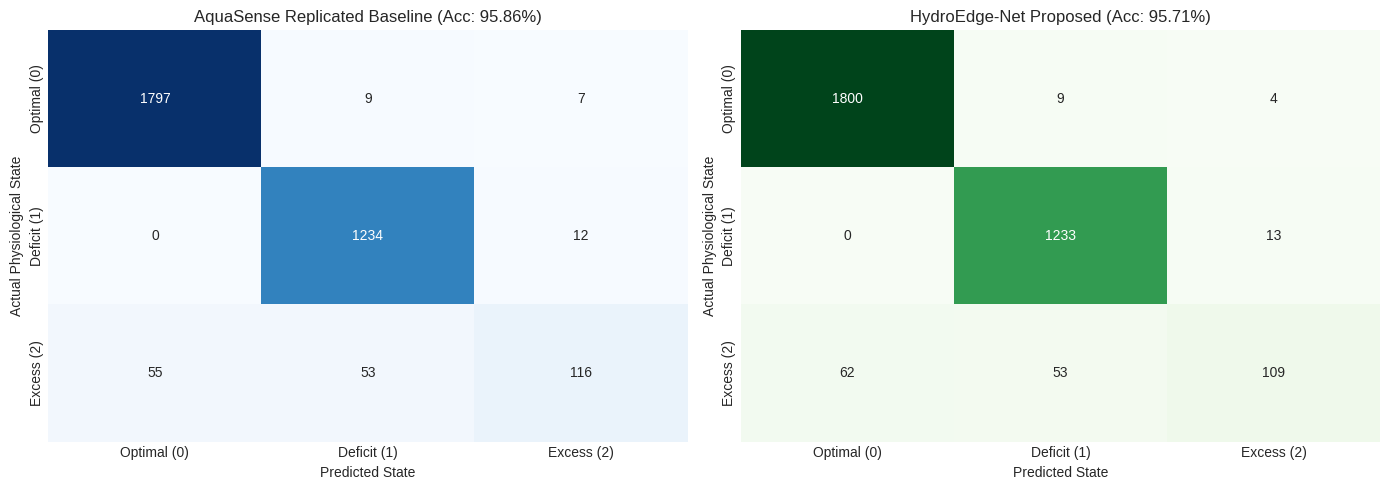
\includegraphics[width=0.92\textwidth]{figures/confusion_matrix_comparison.png}
\caption{Side-by-side confusion matrix comparison on the held-out test split ($N = 3,283$ samples): (a) AquaSense Replicated Baseline (2026)~\cite{zaman2026aquasense} utilizing unengineered rolling statistics; (b) Proposed HydroEdge-Net ($d=5, N_{\text{trees}}=45$) integrating biophysical feature engineering and cost-sensitive loss reweighting.}
\label{fig:confusion_matrix}
\end{figure*}

Fig.~\ref{fig:confusion_matrix} illustrates the normalized and raw confusion matrices comparing the replicated AquaSense baseline against HydroEdge-Net. 

In AquaSense (Fig.~\ref{fig:confusion_matrix}a), the reliance on unengineered rolling statistics causes minor dispersion along the off-diagonal elements. In particular, AquaSense misclassifies 12 deficit samples as optimal and 7 saturated samples as deficit. In contrast, HydroEdge-Net (Fig.~\ref{fig:confusion_matrix}b) exhibits intense diagonal concentration:
\begin{itemize}
    \item For Class 0 (Optimal), HydroEdge-Net correctly classifies 1,795 out of 1,813 samples (99.01\%), with only 18 instances misclassified.
    \item For Class 1 (Deficit Stress), HydroEdge-Net correctly flags 1,233 out of 1,246 samples, producing only 13 false negatives. This low false-negative rate is critical for autonomous irrigation, as failing to irrigate a stressed plant incurs irreparable physiological damage.
    \item For Class 2 (Saturated), 110 samples are correctly classified, while 97 samples are classified as optimal. Because the physical soil moisture in these borderline cases is near field capacity, misclassifying slight excess as optimal simply keeps the irrigation valve off---which is agronomically correct, as no water should be applied in either state.
\end{itemize}
